This lecture introduces more manifold learning algorithms including
Isomap, LLE, LE, MVU and briefly mentions an analog of JL-lemma in the
manifold setting. 

\section{Non-Linear Dimensionality Reduction}
\textbf{Idea}: underlying data follows some kind of manifold.\\
Agenda for today:
\begin{itemize}
\item Isomap (Isometric mapping)
\item LLE (Locally Linear Embedding)
\item LE (Laplacian Eigenmaps)
\item MVU (Maximum Variance Unfolding)
\item Some open problems and approaches to solve these problems
\end{itemize}

\subsection{Isomap}
\subsubsection*{Goal}
Preserve geodesic distances globally. Applications: computer vision. 

\subsubsection*{Notation}
Input data is $X \in \mathbb{R}^{D\times n}$. Output data $Y \in
\mathbb{R}^{d\times n}$ where $d\ll D$. 

\subsubsection*{How?}
\begin{itemize}
\item Approximate the geodesic distances by computing the shortest
  path on a $k$-nearest neighbor ($k$-NN) graph on the input data
  (note that the graph needs to be connected). 
\item Construct a ``distance" matrix $D^{(G)}_{n\times n}$.
\item Run (classical/metric) MDS (multidimensional scaling) to find
  the corresponding embedding ($\min_{Y} \sum_{i<j}||y_i - y_j|| -
  D^{(G)}_{ij}$). 
\end{itemize}

\begin{figure}
\centering
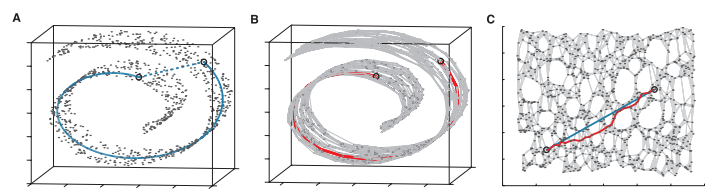
\includegraphics[width=0.5\textwidth]{chapter_7/files/isomap.png}
\caption{Illustration of geodesic distance}
\end{figure}

\subsubsection*{Observations}
\begin{itemize}
\item How well can $k$-NN graph approximate the geodesics.
  \begin{itemize}
  \item Under suitable distributions over the underlying    manifold,
    as $r\rightarrow 0$, $n\rightarrow \infty$, $nr \rightarrow
    \infty$, can show the shortest path $\rightarrow$ geodesic path. 
  \end{itemize}
\item When can geodesic paths become Euclidean paths?
  \begin{itemize}
  \item Underlying manifold needs to be (globally) isometric to some
    $\mathbb{R}^n$; that is, it has no intrinsic curvature. For
    example, a spherical cap (a hemisphere) cannot be embedded into
    Euclidean space without distorting distances (imagine trying to
    flatten the northern hemisphere of a globe without
    stretching/ripping the map).  
  \item Parametrization space should be convex. For example, if there
    is a missing/hole at the center of a manifold, an embedding will
    `fill in' the space and shorten the distance between two points
    that were originally across each other in the original manifold. 
  \end{itemize}
\end{itemize}


\subsection{LLE (Locally Linear Embedding)}
\subsubsection*{Motivation}
Isomap works well under certain conditions - but these conditions will not always hold. We need other algorithms that are capable of handling cases in which the manifold is not isometric to simple Euclidean space.

\subsubsection*{Goal}
Rather than attempting to preserve global geometry as Isomap does, we will instead find a low-dimensional embedding that preserves ``local geometry". But just what is local geometry?

\noindent \textbf{Answer}: Intuitively speaking, a manifold is some object that is locally ``flat" - if you zoom in closely enough, it looks like flat Euclidean space.

If a manifold is locally linear, then one can define ``local geometry" to be how a specific data point is linearly related to its neighbors. That is, every point in our observation set can be viewed as (approximately) a linear combination of its neighbors.

Using this particular definition of ``local geometry", we can find a low-dimensional embedding $Y$ of the given data $X$ such that the locally linear relationships between neighbors are approximately preserved - this is the LLE algorithm.

\subsubsection*{How?}
In overview - given input data $X\in \mathbb{R}^{D\times n}$, number of neighbors
$k$, embedding dimension $d$, we perform the following steps:

\begin{enumerate}
\item First we construct the $k$-NN graph (ideally, a connected graph) to find the nearest neighbors for each data point $x_i$; we denote the set of the $k$ nearest neighbors of $x_i$ as $N_i$, or $N(i)$ (but we'll prefer the latter, since the symbol $N_i$ will be used to refer to something different later).

\item Next, we find the linear representation of each data point using its neighbors with minimum discrepancy to the actual location: we take the minimum over all possible weightings of neighbors for all points

\begin{align*}
\min\limits_{W} \Phi(W) &= \sum\limits_{i=1}^n \bigg|\bigg|x_i - \sum\limits_{j\in N(i)} w_{ij} x_j\bigg|\bigg|^2\\
\text{ s.t. } & \forall i, \sum_{j} w_{ij}=1,\\
& \forall i, w_{ij}=0 \text{ for } j \not \in N(i),
\end{align*}

where $W$ is the weight matrix where entry $W_{ij} = w_{ij}$ is the weight of point $x_j$ in the linear neighbor representation of point $x_i$ (we set $w_{ij}$ to zero if $x_j$ is not a neighbor of $x_i$; and we require that the weights in the neighbor representation of any single point sum to one simply so that we may specify a unique, reasonably-scaled solution).

\item Finally, we find the low-dimensional representation that most closely fits the linear relationship of a point to its neighbors that we found in the previous step:

\begin{align*}
&\min_{Y} \Psi(Y) = \sum_{i=1}^{n} ||y_i - \sum_{j\in N(i)} w_{ij}
  y_i||^2\\ 
&\text{s.t. } Y Y^\intercal = I
\end{align*}

Here, $y_i \in \mathbb{R}^d$ is the embedding of $x_i \in \mathbb{R}^D$.
\end{enumerate}

\subsubsection*{Some notes.}
First - in step 2, why are we solving for the representation of a point by its neighbors as an optimization problem? Why not find the precise solution directly?

As it turns out, not all points \textit{can} be represented exactly as a linear combination of their neighbors. For example, in a very degenerate case, imagine we have three points sitting along a convex curve - let's call them $A, B, C$ for convenience, where $B$ lies between its neighbors $A$ and $C$. Then there's actually no way to represent $B$ as a linear combination of $A$ and $C$ - we can only represent points on the line $AC$, which cuts through the curve! (Try drawing it out if that doesn't make sense.) Another example given in class is a data point at the corner of some space. The 2D case is shown in the figure below.

Similarly, in higher-dimensional space, it's possible for all the neighbors of point $x$ to lie along (or approximately along) some subspace not containing $x$, in which case we won't be able to find an exact solution (or the ``exact" solution will involve some very large coefficients, which will effectively be just an artefact of how we happened to sample the neighbors).

\begin{figure}[H]
\centering
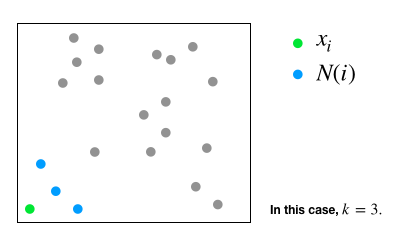
\includegraphics[width=0.5\textwidth]{chapter_7/files/no_linear_comb_case.png}
\end{figure}

\subsection*{Details}
\subsubsection*{Step 2}
Consider the $i^\text{th}$ data point in isolation. For this single point, we'd like to minimize $\Phi (W_{i:})=||x_i-\sum_{j\in N(i)} w_{ij} x_j||^2$. So how specifically will we do this?

First let's define some notation.

\[N_i=
\begin{bmatrix}
    x_{j_1} & x_{j_2} & \dots & x_{j_k} \\
\end{bmatrix};
\]

\[w_i=
\begin{bmatrix}
    w_{ij_1} \\
    w_{ij_2} \\
    \vdots \\
    w_{ij_k} \\
\end{bmatrix}, \text{ and }
e=
\begin{bmatrix}
    1 \\
    1 \\
    \vdots \\
    1 \\
\end{bmatrix}.
\]

Note for clarity that $N_i$ is a $D \times k$ matrix, and $w_i$ and $e$ are $k \times 1$ vectors; the $j_1 \dots j_k$ in $w_i$ are the $k$ neighbors in $N(i)$.

Going back to our original minimization expression, we can rewrite the right-hand term as
\[
\sum_{j\in N(i)} w_{ij} x_j=N_i w_i.
\]

Easy enough. But what about the left-hand term?
\[
x_i = x_i e^{\intercal} w_i.
\]
``What?" you may be saying to yourself. What is this black magic? But you can verify it for yourself: because of our handy assumption that $\sum_j w_{ij} = 1$, the expression $e^\intercal w_i$ can be rewritten as
\[
e^\intercal w_i = \begin{bmatrix}
    1 & 1 & \dots & 1 \\
\end{bmatrix} w_i =
\begin{bmatrix}
    w_{ij_1} + w_{ij_2} + \dots + w_{ij_k} \\
    w_{ij_1} + w_{ij_2} + \dots + w_{ij_k} \\
    w_{ij_1} + w_{ij_2} + \dots + w_{ij_k} \\
    \text{etc.}
\end{bmatrix} =
\begin{bmatrix}
    1 \\
    1 \\
    \vdots \\
    1 \\
\end{bmatrix}.
\]

Using these rewritten terms, it follows that:
\begin{align*}
\Phi (W_{i:})
&= ||x_i e^\intercal w_i - N_i w_i||^2\\
&= ||(x_i e^\intercal-N_i)w_i||^2\\
&= w_i^\intercal (x_i e^\intercal-N_i)^\intercal (x_i e^\intercal - N_i) w_i.
\end{align*}

Now let's pause for a moment. This looks perhaps a bit complicated - but let's focus on just the middle section $(x_i e^\intercal-N_i)^\intercal (x_i e^\intercal - N_i)$. We know $x_i$ and $N_i$, and $e$ is fixed. So this entire expression in fact comes out to a known $D \times D$ matrix! Let's call it $G$. Then our optimization problem is
\begin{align*}
&\min_{w_i} w_i^\intercal G w_i \text{ where } G = (x_i e^\intercal-N_i)^\intercal (x_i e^\intercal - N_i)\\
&\text{s.t. } e^\intercal w_i = 1.
\end{align*}

(Note: at this point one might be tempted to reach for our familiar Rayleigh quotient minimization/minimum eigenvalue solution, but we can't use that here - that requires the condition $w_{i}^\intercal w_i = 1$, which we don't have.)

From here, we relax the constraint using Lagrange and take the derivative of the cost function as follows:
\begin{align*}
L(W_i,\lambda) &= W_i^\intercal G W_i - \lambda (e^\intercal W_i - 1)\\
\frac{\partial L}{\partial W_i} &= 2GW_i - \lambda e = 0\\
\Rightarrow 2GW_i &= \lambda e.
\end{align*}
If $\lambda$ is known, $w_i=G^{-1} \frac{\lambda}{2} e$. But we don't actually know $\lambda$ beforehand! Luckily, knowing $\lambda$ is not necessary: we can pick any $\lambda \neq 0$ and solve for $w_i$, and if we used something other than the true $\lambda$, this will give us a scaled version $w_{i}'$ of the true $w_i$. Recalling again that $\sum_j w_{ij} = 1$, we can normalize $w_{i}'$ to get $w_i = \dfrac{w_{i}'}{\sum_j w_{ij}'}$.

\subsubsection*{Step 3}
We consider the $i^\text{th}$ data point's embedding $y_i$. For this single point, we'd like to minimize $\Psi (y_i)=||y_i-\sum_{j\in N(i)} w_{ij} y_j||^2$.

We define the following notation:
\[Y=
\begin{bmatrix}
    y_1 & y_2 & \dots & y_n \\
\end{bmatrix}
\]
\[
W=
\begin{bmatrix}
    && && \\
    && W_{ij} && \\
    && && \\
\end{bmatrix}, \text{ where } W_{ij} = w_{ij};
\]
and $I$ is the identity matrix.

Note that here, $Y$ is a $d \times n$ matrix; both $W$ and $I$ are $n \times n$ matrices.

We use the subscript $_{:i}$ to refer to a column vector that is the $i^\text{th}$ column of a matrix. So $W_{:i}$ is the $i^\text{th}$ column of $W$, and $I_{:i}$ is the $i^\text{th}$ column of $I$.

Again we can do some rewriting:
\[
y_i = Y I_{:i}
\]
\[
\sum_{j\in N(i)} w_{ij} y_j = Y W_{:i}
\]

so for an individual point with embedding $y_i$, we can write
\[
\Psi (y_i) = ||Y I_{:i} - Y W_{:i}||^2.
\]

Summing over $i$, we can express the overall $\Psi$ term as:
\begin{align*}
\Psi(Y)
&= \sum\limits_{i=1}^n ||Y(I_{:i} - W_{:i})||^2 \\
&= ||Y (I - W)||_F^2 \\
&=\text{Tr}((I-W)^\intercal Y^\intercal Y (I-W)) \\
&=\text{Tr}(Y(I-W)(I-W)^\intercal Y^\intercal).
\end{align*}

The optimization problem becomes:
\begin{align*}
&\min_Y \text{ Tr}(YMY^\intercal) \text{ where } M = (I-W)(I-W)^\intercal \\
&\text{s.t. } Y Y^\intercal=I
\end{align*}

Observe that $Y Y^\intercal=I$ does not exactly fit the generalized eigenvalue problem formulation; we can take $Z = Y^\intercal$ so the formulation becomes:
\begin{align*}
&\min_Z \text{ Tr}(Z^\intercal MZ) \text{ where } M = (I-W)(I-W)^\intercal \\
&\text{s.t. } Z^\intercal Z=I
\end{align*}

We can solve this by taking the eigenvalue decomposition of $M$, and then takes the  $2^\text{nd},3^\text{rd},...,d+1^\text{th}$ eigenvectors.

\subsubsection*{Some observations about LLE.}
\begin{itemize}
\item It does not preserve the scale in the low-dimensional parametrization.
\item It works quite poorly in practice.
\item $(I-W)(I-W)^\intercal$ is kind of like a Laplacian of the underlying graph.
\end{itemize}

\subsection*{LE (Laplacian Eigenmaps)}
\subsubsection*{Goal}
Find a Low-Dimensional embedding of the original input data that preserves ``local geometry" in terms of maximally preserving similarity
between points. 
\textbf{Question}: How do we measure similarity?\\
\textbf{Answer}: Can estimate local distances define similarity
proportional to the distance. 
\subsubsection*{How?}
\begin{itemize}
\item Define $W_{ij}=e^{-||x_i-x_j||^2}{2\sigma^2}$.
\item 
\begin{align*}
&\min_{Y} \sum_{i,j} W_{ij} ||y_i-y_j||^2\\
&\text{s.t. } Y^\intercal Y=I
\end{align*}
$\Rightarrow$
\begin{align*}
&\min_{Y} \text{tr} (Y^\intercal LY)\\
&\text{s.t. } Y^\intercal Y=I
\end{align*}
\end{itemize}
\subsubsection*{Observations}
If points $x_i$ and $x_j$ are far apart, $W_{ij}$ is close to 0 so
$y_i$ and $y_j$ can be mapped anywhere. If $x_i$ and $x_j$ are close,
then $w_{ij}$ is large so it encourages $y_i$ and $y_j$ to be mapped
close. In this sense, it is local neighborhood preserved. 

\subsection*{Discussion}
We can put most linear dimensionality reduction algorithms in a
unified framework. Essentially, they are all special cases of
Kernel-PCA. 
\begin{itemize}
\item PCA: $K=X^\intercal X$(Linear Kernel).
\item Classical-MDS: $K=\frac{-1}{2} HD^{Euclidean}H$ where $H$ is the
  centering matrix. 
\item Isomap: $K=\frac{-1}{2} HD^{Geodesic}H$.
\item LLE: once $W$ is learned, $K=M^{-1}$ or $K=(\lambda_{max} I -
  M)$, where $M=(I-W)(I-W)^\intercal$. (Difference is in the scale of
  coordinate of the embedding. $K=\wedge^{1/2} V$). 
\item LE: $K=L^{-1}$ or $K=(\lambda_{max} I - L)$ and the result is
  also off in the scale of coordinate of the embedding as LLE. 
\end{itemize}

\subsection*{MVU(Maximum Variance Unfolding) (aka. Semi-Definite Embedding(SDE))}
\subsubsection*{Goal} Find a low-dimensional embedding of the given
data which preserves "local geometry" in terms of finding the best
kernel.\\
Define Local Geometry in terms of distance between data points in a
local neighborhood. Denote $D\times n$ matrix
\[
X=
\begin{bmatrix}
    x_1 & x_2 & \dots & x_n \\
\end{bmatrix}
\]
and denote $d\times n$ matrix
\[
Y=
\begin{bmatrix}
    y_1 & y_2 & \dots & y_n \\
\end{bmatrix}.
\]
Want: If $j$ is a neighbor of $i$,
\begin{itemize}
\item \begin{align*}
||x_i - x_j||^2
&=||\phi (x_i)-\phi (x_j)||^2\\
&=K_{ii}+K_{jj}-2K_{ij}
\end{align*}.
\item $K$ is positive semi-definite.
\item $\sum_{ij} K_{ij}=0$.
\end{itemize}

The optimization problem can be formulated as the following:
\begin{align*}
&\max_{K} \text{tr}(K)\\
&\text{s.t. } K_{ii}+K_{jj}-2K_{ij}-||x_i-x_j||^2 \text{ if }i \text{
    and } j \text{ are neighbors}.\\ 
&\text{s.t. } \sum_{ij}K_{ij}=0\\
&\text{s.t. } K \succeq 0
\end{align*}
This is a convex optimization and can find a globally optimal solution.

\subsection*{More discussions}
Suppose we want to preserve geodesic distance approximately.
\begin{theorem}[JL-manifold]
Say n-dimensional manifold $M$ in $\mathbb{R}^D$. We know that the
volume of the manifold, Vol$(M)=V$ and global bound on curvature
$K(M)=k$. $\exists f: \mathbb{R}^D \rightarrow \mathbb{R}^d$ where
$d=O(\frac{n}{\epsilon^2}\log (Vk) )$. $\forall p,q \in M$ and
$G(p,q)$ is the geodesic path between $p,q$. Let $L(\cdot)$ be the
"length" function. $\forall p,q,n$, 
\[
1-\epsilon \leq \frac{L(G(f(p),f(q)))}{L(G(p,q))} \leq 1+\epsilon
\]
$f$ is linear (can use random projection matrix).
\end{theorem}
